% !TEX root = ../../teaching_online.tex
\newpage
\section{Other Resources}

% OCW
\subsection{MIT Open Courseware}

MIT Open Courseware is vast collection of course materials from MIT. Licensed under a \href{https://creativecommons.org/licenses/}{Creative Commons License}, these provide amazing opportunity for students and instructors alike. For students, the site provides an opportunity to learn from a large collection of materials from a diverse selection of courses. For an instructor, it can provide ideas for your own courses, give an extra materials to use with your students, or offer another source of lecture videos (when available). You are able to search courses by department or by available content. Lecture videos can be watched on the main OCW page \url{https://ocw.mit.edu} or on their YouTube page \url{https://www.youtube.com/user/MIT}. 

	\begin{figure}[!ht]
	\centering
	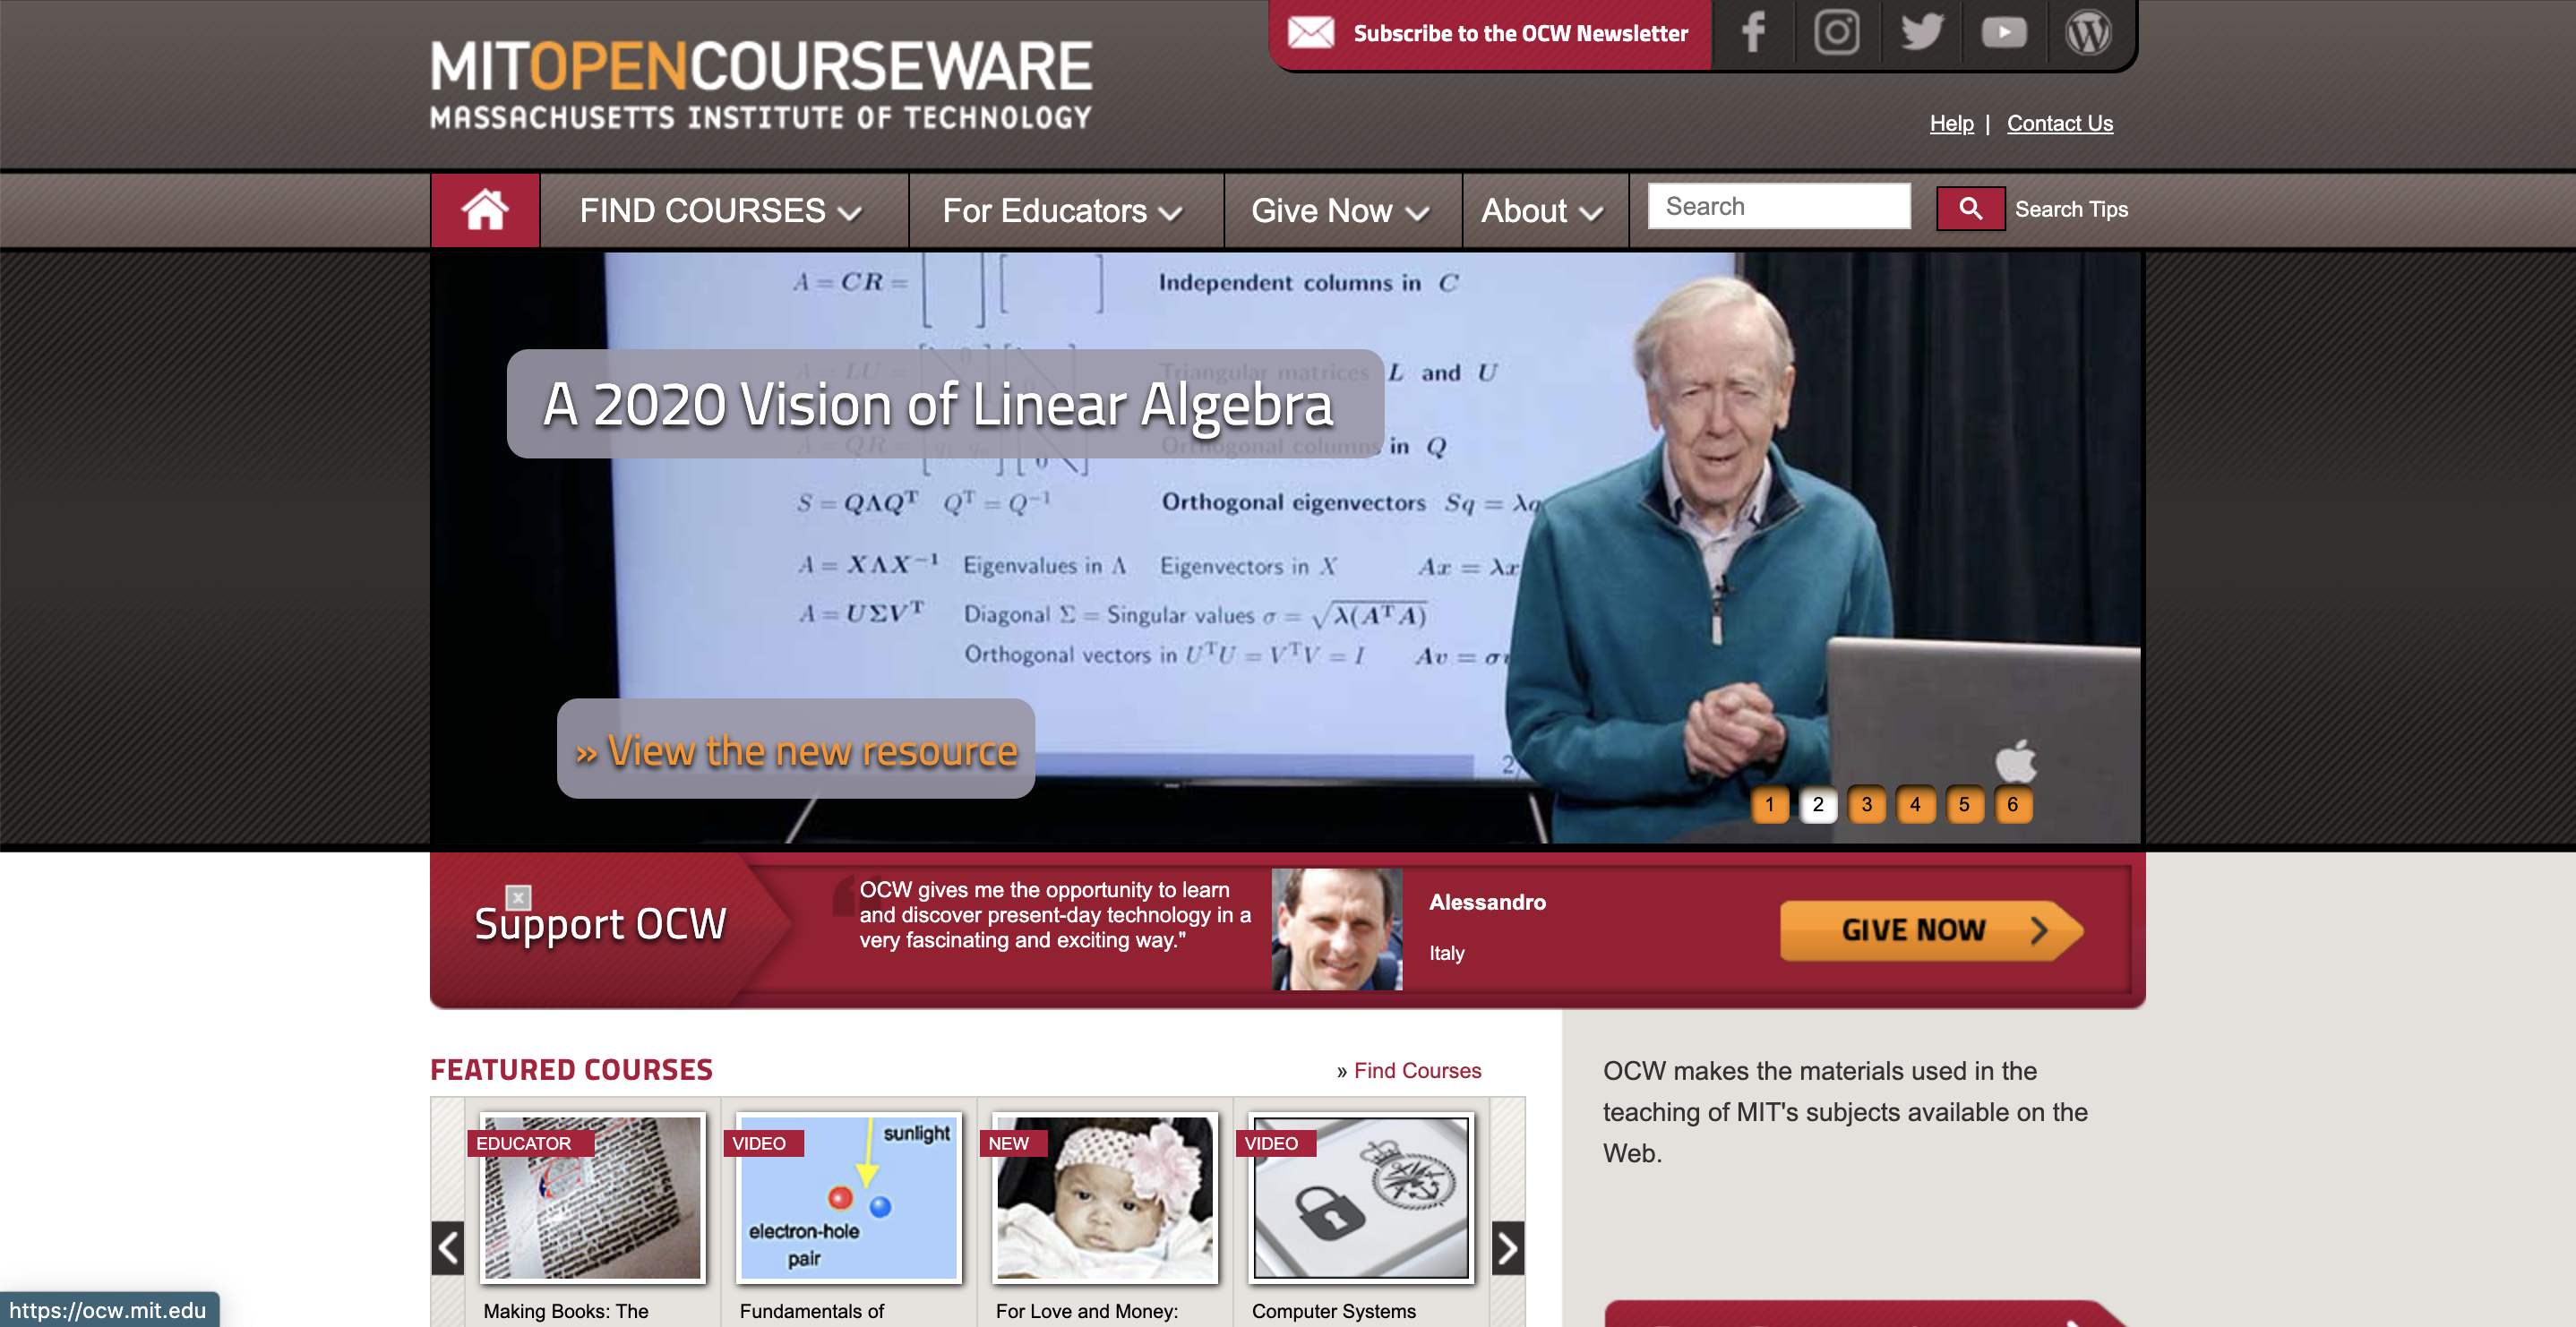
\includegraphics[width=\textwidth]{sections/other/images/ocw.png}
	\caption{MIT Open Courseware.}
	\end{figure}

In particular, OCW has very useful courses for graduate instructors and lab/teaching assistants in STEM. For those graduate students in STEM, we would encourage you to go through the materials and especially the lectures in \its{8.395J Teaching College-Level Science and Engineering (Spring 2009)} and \its{8.395J Teaching College-Level Science and Engineering (Fall 2015)}. These are wonderful lectures covering teaching in STEM specific to college level STEM. 

	\begin{figure}[!ht]
	\centering
	
\includegraphics[width=\textwidth]{sections/other/images/teaching.png}
	\caption{OCW's Teaching College-Level Science and Engineering.}
	\end{figure}

The playlist for the YouTube lectures for these courses can be found at \url{https://www.youtube.com/watch?v=S9uGFKoRGUU&list=PLB1304385546D6F86} and \url{https://www.youtube.com/watch?v=Zm8uMV5aMdw&list=PLUl4u3cNGP60bTiL2hg0h_akgz8ywXkCX}. 



% WolframAlpha
\subsection{Symbolab \& WolframAlpha}

Symbolab and WolframAlpha are symbolic calculators freely available online. Symbolab can be found at \url{https://www.symbolab.com/} and WolframAlpha can be found at \url{https://www.wolframalpha.com/}. These allow the user to enter things like
	\[
	\begin{aligned}
	\dfrac{d}{dx}& \sqrt[3]{x^5} &&& \int_1^3 &(x^3+2x+1) \;dx \\
	\text{Solve } &3x+4= 5 &&& \sum_{n=1}^{10} &n(n+1) \\
	e^{3.2}& &&& \text{Solve } E&= \dfrac{1}{2} L^2 \omega^2 \text{ for } \omega
	\end{aligned}
	\]

This becomes very useful for students who may not have access to (often very expensive) calculators. Moreover, WolframAlpha serves as much more. It can be used as a computational device for many fields, including personal health, engineering, Earth Sciences, Food \& Nutrition, Statistics, etc. It can also interpret, retrieve, and compute with more generic inputs. For example, you can enter
	
	\begin{itemize}
	\item Scrabble score `muzjiks' 
	\item US GDP/US Population
	\item France GDP/US GDP
	\item Temperature Syracuse, NY October 22, 1996
	\item Location international space station
	\item Auriga Seamount relief map
	\item metabolic rate, female, 25y, 5'7'', 130lb
	\end{itemize} 

WolframAlpha (a linguistic `baby' version of the real program Mathematica, which is \href{https://answers.syr.edu/display/ecs/Software}{available to Syracuse University students} for free but does require programming skills), can also take certain Mathematica commands to extend its utility. See THIS DOCUMENT for more information. 

Instructors and teaching assistants alike should be aware of these and other similar websites. These not only will perform computations for students, but will show the steps. Symbolab shows steps (whenever possible) for free, while WolframAlpha requires monthly membership for this service. However last known, the smartphone app version of WolframAlpha will show steps for free without having an account. These and other similar applications could present an opportunity for students to pass off work performed by a computer as their own. Instructors should be aware of the methods these programs use (so that it is easier to recognize suspicious submissions), and consider these and other applications students may take advantage of when creating course assignments. 



% Poll Everywhere
\subsection{Classroom Polling}

Whether teaching online, polling student opinion or questioning students on a topic is a great way to improve classroom participation, increase classroom learning, and help understand what students are thinking/feeling/learning/understanding. There are many ways to can integrate polling into your classroom. There are many options:
	
	\begin{itemize}
	\item \href{https://help.blackboard.com/Learn/Instructor/Tests_Pools_Surveys}{Blackboard} (which can do polls or surveys on the main class page or while using Blackboard Collaborate)
	\item \href{https://www.polleverywhere.com/}{Poll Everywhere} (Free Account: Unlimited questions, 25 max audience, web or smartphone)
	\item \href{https://www.google.com/forms/about/}{Google Forms} (free, online surveys)
	\item \href{https://kahoot.com/}{Kahoot!} (survey/polls/questions, web or smartphone)
	\item \href{https://socrative.com/}{Socrative} (survey/polls/questions, web or smartphone)
	\item Others: \href{https://www.gosoapbox.com}{GoSoapBox}, \href{https://goformative.com}{Formative}, \href{http://www.micropoll.com}{Micropoll}, \href{https://www.poll-maker.com}{PM}
	\end{itemize}



% Jeopardy
\subsection{Jeopardy!}

Jeopardy! is a television game show in which contestants answer clues which are given as answers and the contestant's answers are given as questions. For example, a clue might be, ``In 1492, Columbus sailed this famous ocean's blue,'' where the answer in this case would be, ``What is the Atlantic Ocean.'' There are a few more aspects to the game: double and final jeopardy, etc. You can read more about the game on its Wikipedia page \url{https://en.wikipedia.org/wiki/Jeopardy!}. These can be a great way for students to interact with course material, whether in the classroom or online (synchronous or asynchronous). There are websites on which you can create your own Jeopardy! games. 

	\begin{itemize}
	\item Jeopardy Labs: \url{https://jeopardylabs.com/}
	\item Factile: \url{https://www.playfactile.com/}
	\end{itemize}



















